\section{Different types of transformations}
There exists different types of transformations which can be performed on images, three of them are \textit{rigid}, \textit{affine} and \textit{non-rigid}. A rigid transformation describes a rotation, an \textit{x} translation and a \textit{y} translation. This means the image can be moved a number of pixels in the \textit{x} and \textit{y} direction along being rotated. This is the simplest transformation, but given it only consists of three parameters it is also the easiest to optimize. The transformation matrix used to describe a rigid transformation would be:
\begin{equation*}
	\begin{bmatrix}
		cos(\theta) & -sin(\theta) & t_x \\
		sin(\theta)  &  cos(\theta) & t_y \\
		0				 & 0				 & 1
	\end{bmatrix}
\end{equation*}
The transformations it can make can be visualized as the top row of \autoref{rigidAffine}. A combination of translation and rotation can also be made.

\begin{figure}[h]
	\centering
	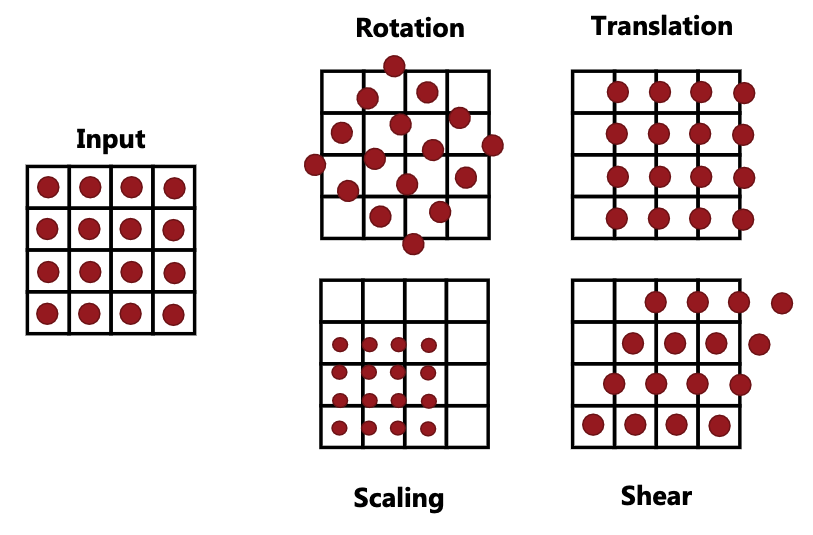
\includegraphics[width=0.75\linewidth]{Materials/affineRigid}
	\caption{Input image along a row of rigid transformations (top) and a row of affine transformations (bottom). Image taken from lecture slides.}
	\label{rigidAffine}
\end{figure}
An affine transformation can in addition to translations and rotations make scaling and shearing effects. Because of this, it requires additional parameters to optimize. The transformation matrix can be written as:
\begin{equation*}
	\begin{bmatrix}
		1+p_1 & p_2 & p_3\\
		p_4  &  1+p_5 & p_6\\
		0				 & 0				 & 1
	\end{bmatrix}
\end{equation*}
The plus 1 are used to ensure we find the identity matrix if the optimal solution is to apply no deformation. The transformations it can make can be seen in \autoref{rigidAffine} where the bottom row is affine transformations. A combination of all aforementioned transformations can also be made.\\
A non-rigid transformation has even more parameters, but can again perform even greater deformations to the image, like circular, curved, arbitrary and stretched transformations. As it has nine parameters it is the hardest of the three transformations to find an optimal solution for. The transformation matrix can be written as:
\begin{equation*}
	\begin{bmatrix}
		1+p_1 & p_2 & p_3\\
		p_4  &  1+p_5 & p_6\\
		p_7	 & p_8	& 1+p_9
	\end{bmatrix}
\end{equation*}
The transformations it can make can be seen in \autoref{nonrigid}. Along these new transformations it can also perform rigid and affine transformations and any combination of the specific transformations. 

\begin{figure}[h]
	\centering
	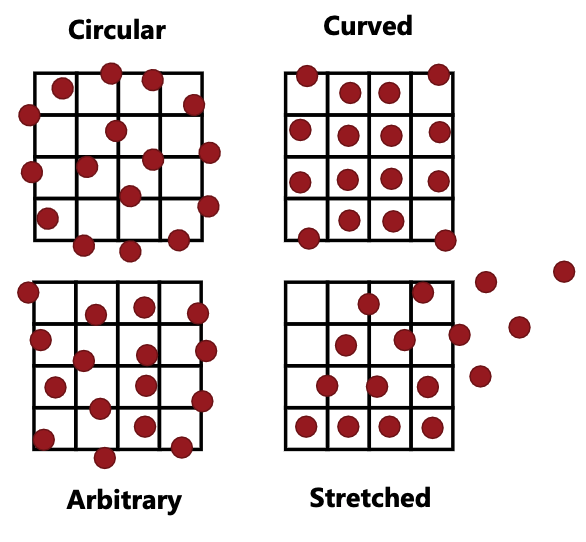
\includegraphics[width=0.55\linewidth]{Materials/noneRigid}
	\caption{Examples of non-rigid transformations. Image taken from lecture slides.}
	\label{nonrigid}
\end{figure}
As the complexity of optimization increases with each additional parameter which needs to be optimized, we use each type of transformations in different contexts. As a rigid transformation can not deform the image, it is often chosen when we have intra-subject images where we expect the scanned object to keep its shape. This could be intra-subject brain MRI, perhaps a follow up scan, as we do not expect the patient's brain to change in shape or size, but we do expect the patient to lie differently in the MRI scanner at each scan. Affine transformations are often chosen when we compare inter-subject images. Here we might want to compare an ill brain to a healthy one, and so we expect small scale differences or small variations in shape. Non-rigid transformations are used when we want to compare object which potentially can have very different shapes. This could be intra- or inter-subject lung CT scans where the patient is breathing while the scan is performed and thus two intra-subject scans might end up very differently. In addition, the shapes of lungs greatly varies between patients, and so strong deformation might be needed to align two lung CT scans.